%%%%%%%%%%%%%%%%%%%%%%%%%%%%%%%% 
\section{The Light Readout System} 
\label{sec:detectors-fd-alt-light}

The baseline assumption in the LAGUNA-LBNO design study was to use for the detection of the scintillation light 8-inch cryogenic photomultipliers (Hamamatsu R5912-02mod) with TPB coating placed below the cathode at about 1m distance. The WA105 demonstrator will use 36 of such photomultipliers (1/$m^2$), the mechanics for the PMTs fixation has been carefully studied in order to contrast the buoancy and do not stress the PMT glass due to the differential in thermal contraction effects between the support and the PMT itself. The application of the TPB coating can be done at the level of the glass itlsef on on a trasparent plate mounted over the photocatode surface.

A 15-20 kt dual-phase liquid argon detector will be equipped with a large number of PMTs which, depending on the PMTs density on the detection surface below the TPC cathode,can reach up to 1000 units. The large number of photosensors calls for an integrated solution for the front-end electronics.
Solutions of this kind have been studied, in the framework of the R\&D program PMm2 \cite{PMM2-1, PMM2-2}, for the instrumentation of giant water
Cherenkov detectors with photomultipliers. The solution developed by this R\&D represents an
important handle for costs reduction. The signal digitization is performed by grouping the
photomultipliers in arrays of 16. Each photomultiplier array is then read out by an ASIC
(Application Specific Integrated Circuit) chip in AMS SiGe 0.35 $\mu$m technology. The ASIC,
which is called PARISROC (Photomultiplier ARrray Integrated in Si-Ge Read Out Chip) 
\cite{Parisroc}, provides a complete readout system for trigger-less acquisition.

\begin{cdrfigure}[Layout of the PARISROC ASIC]{parisroc}{Layout of the PARISROC ASIC used for the production of the second iteration of the
chip. (from Nucl.Instrum.Meth. A623 (2010) 492-494).}
 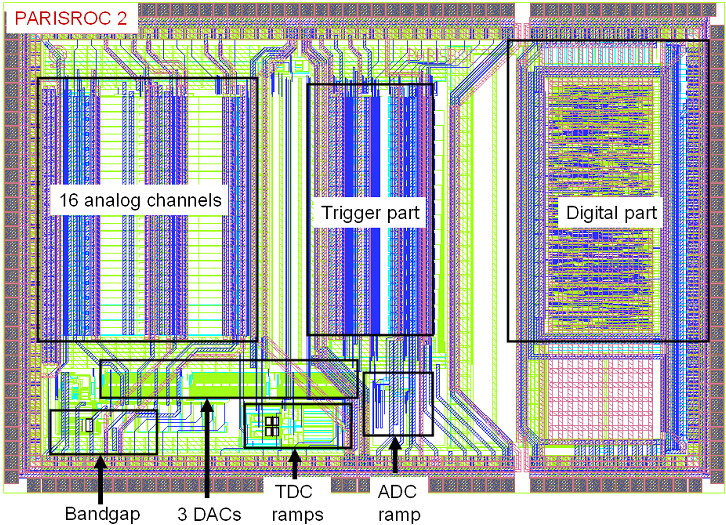
\includegraphics[width=.6\textwidth]{PARISROC2}  
\end{cdrfigure}

The frond-end electronics for the light readout of the DLAr detector will be based on the solution 
developed within the PMm2 R\&D. The PARISROC ASIC, as described in the following, is currently adapted to the 
time structure of the scintillation light produced in the interactions of secondary particles in neutrino interactions in LAr. 
The detection of the direct scintillation light (S1) is the main purpose of the electronics in order to provide the absolute time.
The electronics will be capable to detect the so-called proportional scintillation light (S2) produced by the electrons extracted and amplified in the gaseous phase.

The PARISROC chip reads the signals of 16 photomultipliers totally independently from each
other. Each analogue channel consists of a low-noise preamplifier with variable and adjustable
gain (8 bits) to compensate the relative photomultiplier gain differences powered by a single high
voltage. The preamplifier is followed by a slow channel for the charge measurement in parallel
with a fast channel for the trigger output. The slow channel includes a variable (50-200 ns) slow
shaper followed by an analogue memory with depth of 2 to provide a linear charge measurement
up to 50 pC; this charge is then converted by a 10-bit Wilkinson ADC. The fast channel is
composed of a fast shaper (15 ns) followed by a low offset discriminator to auto-trigger down to
10 fC. This auto-trigger feature makes the PMT array completely autonomous from the other
PMT arrays. The threshold is loaded by an internal 10-bit DACs common for the 16 channels.


\begin{cdrfigure}[Block diagram of the PARISROC ASIC.]{block-diag}{Block diagram of the PARISROC ASIC.}
 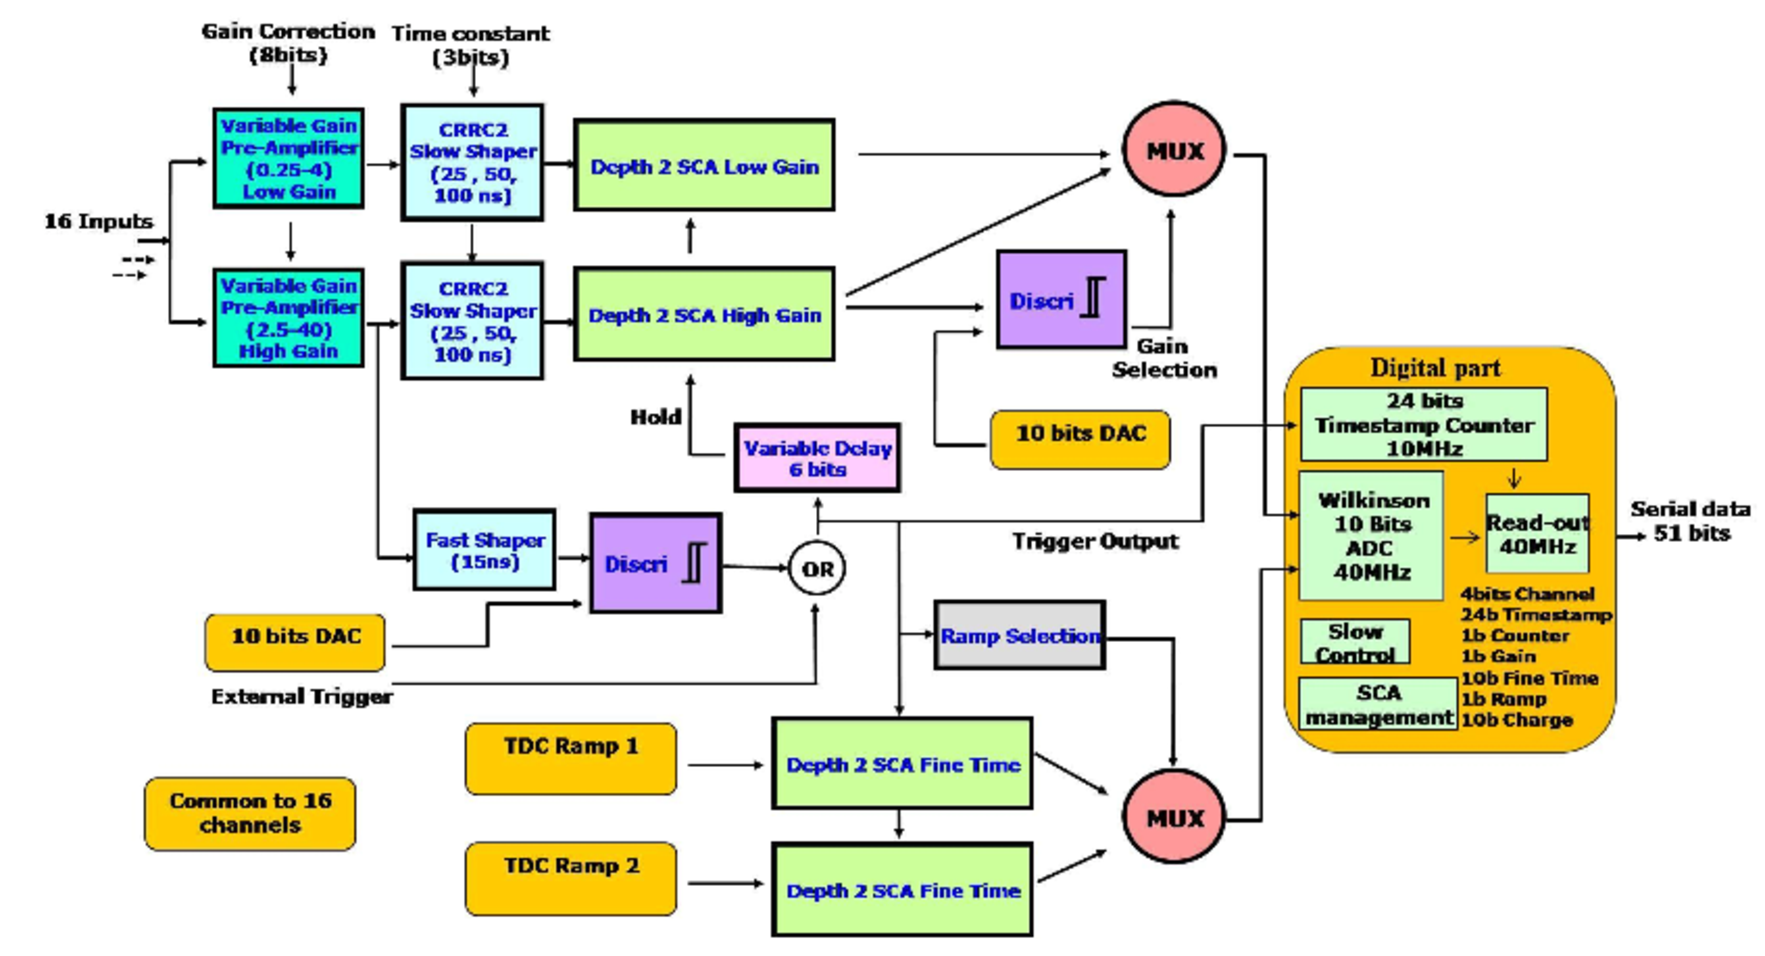
\includegraphics[width=.6\textwidth]{parisroc_blockdiag.pdf}  
\end{cdrfigure}


The variable gain of each pre-amplifier provides the flexibility to adapt the system to the caracteristics of each individual photomultiplier after they have been correcly calibrated. Regarding the timestamping process, there are two TDC ramps working in phase opposition, this way, the dead time when the ramp goes to zero is reduced by selecting the other ramp, that will be in its linear state. Then, when an event arrives, the value of the correct ramp is digitized and inserted in stream of data that includes: a 24 bits counter that goes much slower than the ramps to have a coarse time measurement, a flag that indiciates wich ramp has been digitized, a ID of the channel triggered and the timestamp and charge information.

\begin{cdrfigure}[MicroTCA rack and Bittware S4AM board]{LRO-rack}{MicroTCA rack and Bittware S4AM board}
 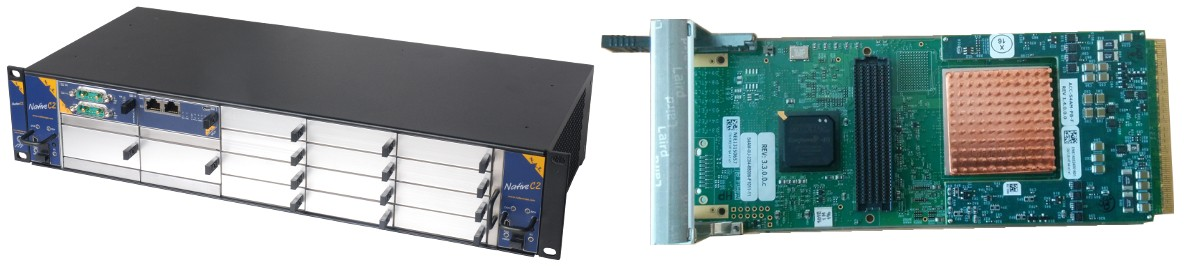
\includegraphics[width=.6\textwidth]{rack}  
\end{cdrfigure}

The light read-out is fully integrated in the DAQ scheme. A microTCA crate (see Figure \ref{fig:rack}) hosting the light readout digitization cards is naturally integrated in this architecture by taking into account the common time distribution and data transmission systems.  During the data taking outside the beam spills a trigger which can be generated by the light readout microTCA crate and its time-stamp can be transmitted over the WR network similarly to the beam trigger. 

There is also an ADC (AD9249 from Analog Devices) that digitizes the charge information for every channel independently. The charge measurement provides information that can be correlated with the one coming from the PARISROC for better precision. A prototype of the light readout AMC is also being realized by still using the Bittware development card S4AM and a mezzanine card including the ADC and the trigger circuit (see Figure~\ref{fig:DAQ-LRO}). 


\begin{cdrfigure}[Block diagram of the light readout AMC demonstrator card]{DAQ_LRO}{Block diagram of the light readout AMC demonstrator card}
 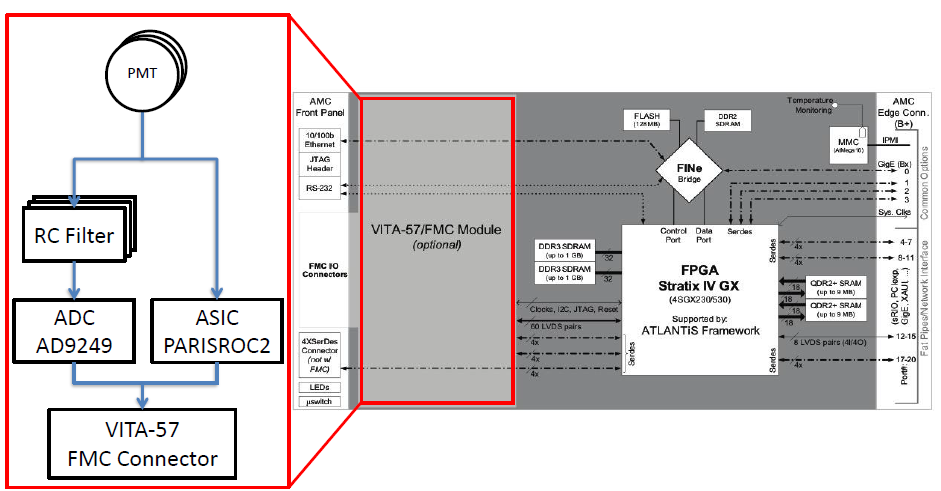
\includegraphics[width=.6\textwidth]{DAQ_LRO}  
\end{cdrfigure}

On this board, the PARISROC chip provides the timestamp at nanosecond level and generates the trigger. In parallel, there is an ADC AD9249 that is continuously digitizing all channels independently at 65 MSPS with 14 bits. The FPGA Stratix IV from the Bittware S4AM card controls and programs the ADC and PARISROC. It also receives the data coming from both PARISROC and ADC. It controls which information will be passed through the network to store it for its analysis. The firmware of the FPGA is in early stages of development and there is still an open debate about which information will be useful. It will definitevely include the timestamp of every event on each channel as well as the digitization of the charge received in each of them. Some questions still in the air are how much charge data is relevant and the feasibility of including some real-time processing. This could include an inverse filter of the RC circuit to compensate its contribution. 

\begin{cdrfigure}[Layout of the mezzanine board]{FEB}{Layout of the mezzanine board}
 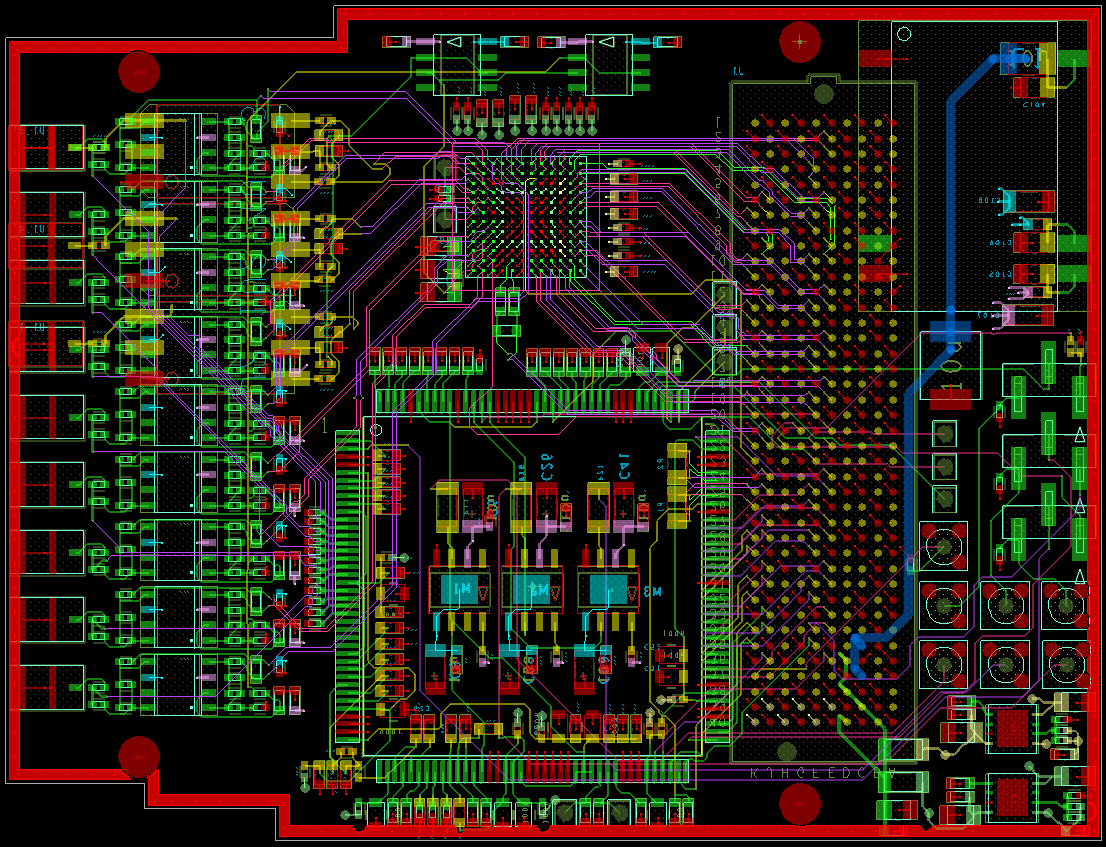
\includegraphics[width=.6\textwidth]{FEB}  
\end{cdrfigure}
 
With this architecture it is possible to achieve a precision of nanosecond at the trigger generation and timestamping of the events. Regarding the charge digitization there is a 14 bits sample every 15ns meaning that considering a 5$\mu$s signal duration, there will be over 300 data points. With this amount of data it is possible to measure not only the total charge generated but also the shape of the signal and decay of the light.
